%====================================================
%	CHAPTER 1 - INTRODUCTION
%====================================================
\chapter{Introduction}
\label{ch:intro}
%====================================================
\section{Foreword}
\label{sec:intro.foreword}
%====================================================
\subsection{A Brief Background to the Study}
\label{subsec:intro.foreword.background}
%====================================================
A popular topic for current control and automation research is that of quadrotor unmanned aerial vehicles (\emph{UAVs}). Attitude control of a quadrotor poses an unique 6-DOF control problem, to be solved with an underactuated 4-DOF system. As a result the pitch, $\phi$, and roll, $\theta$, plants are not directly controllable. The attitude plant is often linearized around a stable operating point. The trimmed operating region is always at the inertial frame's origin; resulting in a zero setpoint tracking problem. The highly coupled nonlinear dynamics of a rigid body's translational and angular motions arise from gyroscopic torques and Coriolis accelerations (Sec:~\ref{subsec:dynamics.nonlinearities.gyrotorques}). Such effects are mostly negligible around the origin, hence the origin trim point decouples the system's nonlinearities. The control system can therefore reduce each first order tracking state variable, $\vec{\mathbf{x}}_b=\big[x~y~z~\phi~\theta~\psi\big]^T$, to independent single-input single-output (\emph{SISO}) plants. Those simplifications are derived in the App:\ref{app:equations.standard}.
\par
As almost every quadrotor research paper mentions, the recent interest in the platform is due to increased availability of micro-electromechanical systems (\emph{MEMS}) and low-cost microprocessor systems. These technical advancements accomodate onboard state estimation and control algorithm processes in real time. Developmental progress in quadrotors and, to a lesser extent UAVs in general, has led to rapidly growing enthusiast communities. For example; HobbyKing\cite{hobbyking} is now a name synonymous with providing custom DIY hobbyist quadrotor assembly kits and frames, no longer retailing only prebuilt commercial products like DJI's Phantom\cite{phantom} or Parrot's AR\cite{parrotar} drones.
\par
The avenue for potential application of both fixed wing and vertical take-off and landing (\emph{VTOL}) UAVs is expansive; supporting civil\cite{civilquadcopter}, agricultural\cite{agriculturequadcopter} and security\cite{videosurveillancequadcopter} industries and not just recreational hobbyists. The quadrotor design provides a mechanically simple platform on which to test advanced aerospace control algorithms. Commercial drone usage in industry is already emerging as a prolific sector; especially in Southern Africa. Subsequently, following the $8^{th}$ amendment of civil aviation laws \cite{dronelaw}, commercial use of UAVs is now both legalized and regulated. Research into any non-trivial aspect of the field will therefore be to extremely valuable to the field as a whole. 
\par
Large scale quadrotor, hexrotor and even octorotor UAVs are popular intermediate choices for aerial cinematography and other high payload capacity applications. The cost of commercial drones such as the SteadiDrone Maverik \cite{steadidrone} is significantly less than a chartered helicopter, used to achieve the same panoramic aerial scenes or on-site inspections. One foreseeable issue which may hinder commercial drone progress in the agricultural and civil sectors is the consequential inertia damping effects from scaling up a vehicle's structure. When increasing the size of any vehicle, its performance is adversely affected if actuation rates are not proportionately increased.
%====================================================
\subsection{Research Questions \& Hypotheses}
\label{subsec:intro.foreword.hypotheses}
%====================================================
The difficulty with quadrotor control is that fundamentally, from their uncertainty and underactuation, they are ill-posed for 6-DOF setpoint tracking. A quadrotor inherently has only four controllable inputs; each propeller's rotational speed $\Omega_{1,2,3,4}$ which are then abstracted to a net virtual control input net torque $\vec{\tau}_\mu=[\tau_{\phi}~\tau_{\theta}~\tau_{\psi}]^T$ and a scalar perpendicular heave thrust projection $\vec{F}_\mu=\sum_{i=1}^{4}~T(\Omega_i)\cdot\hat{z}_b$ in the $\hat{Z}_b$ direction. Those four inputs are then used to effect both the translational XYZ positions $\vec{\mathcal{E}}_I=[x~y~z]^T$ and angular pitch, roll and yaw attitude rotations $\vec{\eta}_b=[\phi~\theta~\psi]^T$. Pitch and roll torques, $\tau_{\phi}$ and $\tau_{\theta}$ respectively, are produced from differential thrusts of each opposing propeller. Yaw torque $\tau_{\psi}$ is induced from the net aerodynamic drag about each propeller's rotational axis. Aerodynamic drag and differential thrust responses are highly nonlinear (detailed later in Sec:\ref{subsec:dynamics.aero.bem}) and difficult to approximate as sources of control action. As a result the body's yaw channel control is depreciated. Stemming from the system's underactuation, the attitude control problem is a zero setpoint problem, attempting to track attitudes is ill-posed and will only ever be locally stable (in the Layupanov sense, Sec:\ref{sec:control.lyapunov}).
\par
\begin{figure}[htbp]
\begin{subfigure}{0.5\textwidth}
\centering
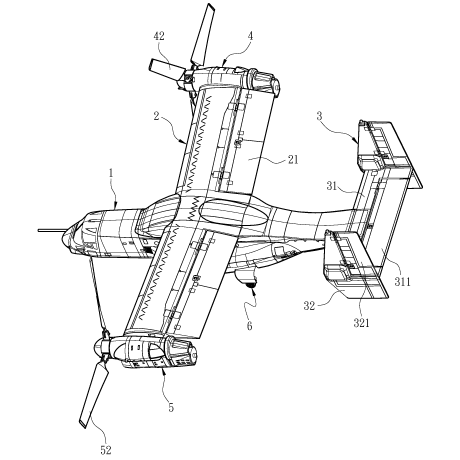
\includegraphics[width=0.85\textwidth]{figs/v22-patent-down}
\caption{Rotors articulated forwards}
\end{subfigure}
\begin{subfigure}{0.5\textwidth}
\centering
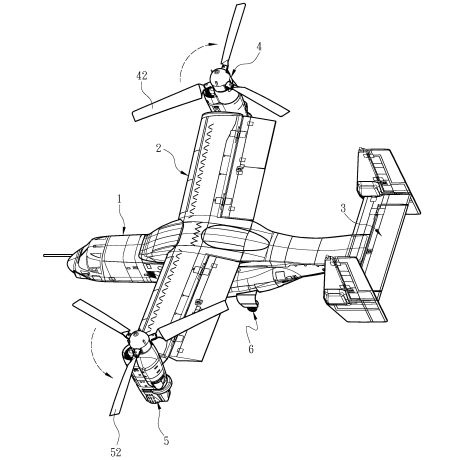
\includegraphics[width=0.85\textwidth]{figs/v22-patent-up}
\caption{Rotors articulated upwards}
\end{subfigure}
\caption{Bell/Boeing V22 Osprey actuation, notations pertinent to patent \cite{ospreypatent}}
\label{fig:osprey}
\end{figure}
The aim of this research is to implement non-zero attitude and position state setpoint tracking on a quadrotor by solving the problem of its inherent underactuation. Inspired by Boeing/Bell Helicopter's V22 Osprey (Fig:\ref{fig:osprey}) and the tilting articulation of its propellers, the prototype design proposed here (described in Sec:\ref{sec:proto.design}) introduces two additional actuators for each of the quadrotor's four lift propellers, specifically adding rotations about the $\hat{X}$ and $\hat{Y}$ axes for each motor/propeller pair. The result is four individually articulated 3-D thrust vectors instead of a bound perpendicular net heave force. The control problem is then posed as the design and allocation of net input forces $\vec{F}_{\mu} = [F_x\;F_y\;F_z]^T$ and torques $\vec{\tau}_{\mu} = [\tau_{\phi}~\tau_{\theta}~\tau_{\psi}]^T$ to act on a general 6-DOF body, such that for any desired trajectory $\vec{\mathbf{x}}_d(t)=[x~y~z~\psi~\theta~\phi]^T$ the error state $\vec{\mathbf{x}}_e(t) \triangleq \vec{\mathbf{x}}_d(t) - \vec{\mathbf{x}}_b(t)$ is asymptotically stable. Mathematically:
\begin{equation} \label{eq:trajectoryerror}
\lim_{t \rightarrow \infty} \vec{\mathbf{x}}_e(t) = \vec{0}~~~~\forall \vec{\mathbf{x}} \in \mathbb{R}^n
\end{equation}
where $n$ is number of the degrees of freedom the system has, typically a 6-DOF plant for rigid bodies. Trajectory stability is explicitly defined later (Sec:\ref{sec:control.stability}) in the context of Lyapunov stability analysis (Sec:\ref{sec:control.lyapunov}). The overactuation brings about the need for a control allocation scheme, one which distributes the six commanded system inputs (net torques and forces) among the twelve actuators in order to optimize some objective function secondary to that of Eq:\ref{eq:trajectoryerror}. The potential improvement(s) for exploiting those overactuated elements is the most novel outcome which the project could yield.
\par
Part of the control research is the multivariable dynamic modelling of the system; making as few assumptions as possible about the nonlinear dynamics involved in the quadrotor's motion and its operational conditions. Common linearizations applied to the quadrotor's control plant will not hold true for more aggressive attitude maneuvers; they are dependent on small angle approximations and neglect second or higher order effects. To produce a stabilizing control solution, there first needs to be a plant model that incorporates both multibody and actuator dynamics, against which the controller efficacy can be tested. The final key outcomes for the project are; the prototype design, its mathematical plant model and simulation analysis, the resultant control law produced and finally conclusions drawn on all of the above.
\par
For a rigidly connected multibody system with revolute joints between sub-bodies, the induced relative motion between those sub-bodies will produce complex dynamics like inertial and gyroscopic responses, amongst others. A rotating propeller will respond to pitching or rolling much like a Control Moment Gyroscope \cite{cmg} or a flywheel, producing a precipitating torque cross product. A less trivial aspect, which is occasionally considered, is the aerodynamic effects produced from the propeller's aerofoil profile. Such induced responses manifest normal to the propeller's rotational axis. Those aspects are not typically compensated for due to a quadrotor's fundamental co-planar propeller counter-rotating pairs which mostly negate such effects. A strongly plant dependent control law is needed for dynamic compensation, reducing potential fragility associated with the subsequent stability proof. Unmodelled dynamics could push the plant out of the range of stability with regards to the Lyapunov proof. 
%====================================================
\subsection{Scope and Limitations}
\label{subsec:intro.foreword.scopeandlim}
%====================================================
\subsubsection{Scope}
\label{subsubsec:intro.foreword.scope}
%====================================================
Critical to this project is the conceptualized design, prototyping and modelling of a novel actuation suite to be used on a quadrotor platform. The control research question is to apply dynamic setpoint control to the quadrotor platform. Stemming from this is an investigation into the kinematics that are potentially influenced by such a design and the structure's configuration changes. In order to apply correct control theory to achieve the state tracking on the physical prototype, plant dynamics must first be identified for the controller to be designed and optimized correctly. Aspects of the mechanical design are detailed in the next chapter, Ch:\ref{sec:proto.design}. There is no scope beyond the cursory investigation for materials analysis or stress testing of the design. This dissertation's scope focuses on deriving the vehicle's equations of motion and subsequent control design, not the structural integrity of the proposed frame given the forces it may undergo. No flight tests were performed but physical measurements were made on the platform for kinematic inertia measurements (Sec:\ref{sec:proto.inertia}) and experiments were conducted for corroboration of second order gyroscopic and inertial dynamic responses relating to the novel actuation block (Sec:\ref{subsec:dynamics.nonlinearities.torque-tests}).
\par
Despite aiming to track first order trajectory setpoints, flight path planning and the trajectory generation thereof are not ubiquitous with this dissertation. Derivations for the differential equations for a 6-DOF body's motion, throughout Ch:\ref{ch:dynamics}, are applicable to any aerospace body, rigid or otherwise. Some particular standards are used, like ZYX Euler Aerospace rotational matrix sequences, all of which are covered in Sec:\ref{sec:proto.conventions}. The control plant is stabilized with nonlinear state-space control techniques in the time domain, aided and justified by Lyapunov stability theorem\cite{noteonlyapunov,nonlinearsystems,bojelayupanov}. Alternative solutions using model predictive control (\emph{MPC}) or quantitative feedback theory (\emph{QFT}) could perhaps yield more refined or effective controllers, however they are not discussed here and remain open to further investigation. Quadrotor attitude control is commonly stabilized with feedback linearizations, decoupling the plant around a trim point so that SISO techniques can be applied. A derivation of such a linearization is included in App:\ref{app:equations.standard} but beyond that there are no further discussions. Any comparisons between non-zero and zero setpoint attitude controller efficacy for quadrotors are difficult as the fundamental objectives are in stark contrast with one another.
\par
Arguably the most important and potentially novel aspect of this project is the control allocation. The system has twelve plant inputs and six output variables to be controlled. There is then an entire set of compatible actuator solutions, $\vec{u}\in\mathbb{U}\in\mathbb{R}^{12}$, which satisfy each commanded virtual input. Such a plant is classified as overactuated. There must be some logical process as to how those twelve actuators are combined to achieve the desired six control plant inputs; specifically input force $\vec{F}_{\mu}$ and torque $\vec{\tau}_{\mu}$ acting on the system.
\par
Appropriate allocation rules are first derived in Ch:\ref{ch:allocation} then simulated and compared in Ch:\ref{ch:simulation} before the final solution is reviewed in Ch:\ref{ch:conclusion}. It is not a comprehensive survey of every possible allocation or control scheme but rather an analysis of the sub-set of problems and design of what is regarded as a logical and pertinent approach. With regards to the prototype design in Sec\ref{sec:proto.design} it is assumed that certain aspects are readily available and require no design/development. Particularly the position and attitude state estimation, which is assumed to be updated through a five-camera positioning system and fused with an on-board 6-axis inertial measurement unit (\emph{IMU}) using some discretized filtration, is assumed to be accurate and readily disposable at a consistent 50 Hz. Hence state estimation and its discretization effects are included in Sec:\ref{sec:simulation.state} but are bereft of intricate detail. State estimation for quadrotors and aerial vehicles is a thoroughly researched subject, \cite{arnold,spacecraftkalman,attitudedetermination}.
%====================================================
\subsubsection{Limitations}
\label{subsubsec:intro.foreword.limits}
%====================================================
The biggest constraint faced by the design is the net weight of the assembled frame. Lift thrusts which are required to keep an aircraft aloft and oppose the net gravitational force are obviously dependent on the body's net weight. The steady state actuator positions and rates ought to be far less than their respective saturation limits to ensure sufficient actuator headroom to implement control actuations. Conversely the structure's net weight is mostly dependent on the lift motors which are often the heaviest part of the vehicle (batteries included). 
\par
A trade-off between net weight and actuator bandwidth/headroom makes designing the prototype a balancing act of compromise; added actuation is needed to produce the desired thrust vectoring. The added actuation increases the weight which then requires more thrust force to ensure the vehicle remains airborne. Larger motors therefore need stronger actuators to effect the rotational motion applied to the sub-bodies to overcome their inertial responses. There is a compromise between the weight of the body and the strength/quality of the actuation.
\par
To forego the deliberation detailed above, reducing the possibility of unbounded scope creep, a design limitation is self-imposed on the prototype design. Restricting the propeller diameter, and hence maximum thrust/frame size, will provide a constraint upon which all other design considerations must adhere to. Smaller propellers require far greater rotational speeds to produce similar levels of thrust than their larger diameter counterparts could provide. Electing to use three bladed $6\times 4.5$ inch diameter propellers constrained the maximal overall dimensions of the prototype; but as a consequence required very high revolution per minute (\emph{RPM}) motors. Specifically a set of four Cobra-2208/2000 KV \cite{cobramotor} brushless direct current (\emph{BLDC}) motors are proposed for lift actuation (Fig:\ref{fig:cobra}). 
\par
A direct consequence of that decision is (provisionally based on official thrust tests of the motor included in App:\ref{app:cobra-test}) the net thrust disposable to the control loop is limited to around $950~\text{g}\approx 9.3~\text{N}$, per motor at $14.1~\text{V}$. That thrust test data is provided from the official Cobra motor's website, \cite{cobramotor}, but further verification is done through physical testing in Sec:\ref{subsec:dynamics.aero.bem}. The frame weight should ideally remain below 50\% of the maximum available thrust, or roughly below $2~\text{kg}$.
\par
Another aspect of limitations produced by design decisions made, mostly to reduce the prototype's cost, is to use of 180\textdegree ~rotation servo motors. Here Corona DS-339MG metal gear digital servos (Fig:\ref{fig:corona}) were selected as they were readily available from university stores. The servos are used for each individual motor's $\hat{X}_{M_i}$ and $\hat{Y}_{M_i}$ axial pitch and roll actuations respectively; terms $\lambda_i$ and $\alpha_i$ represent those respective rotations for the $i^{\text{th}}$ motor set to differentiate from body pitch $\phi$ and roll $\theta$.
\par
\begin{figure}[hbtp]
\vspace{-4pt}
\begin{subfigure}{0.5\textwidth}
\centering
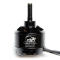
\includegraphics[width=0.8\textwidth]{figs/cobra-motor}
\vspace{-6pt}
\caption{Cobra CM2208/2000KV BLDC motor~\cite{cobraimage}}
\label{fig:cobra}
\end{subfigure}
\begin{subfigure}{0.5\textwidth}
\centering
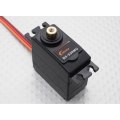
\includegraphics[width=0.8\textwidth]{figs/corona-servo}
\vspace{-6pt}
\caption{Corona DS-339MG digital servo~\cite{hobbyking}}
\label{fig:corona}
\end{subfigure}
\vspace{-8pt}
\caption{Mechanical actuators}
\vspace{-14pt}
\end{figure}
\par
Servos act in place of either BLDC gimbal or stepper motors with closed loop position control to articulate actuator rotations. The latter pair could both accommodate for continuous ($>2\pi$) rotations of the actuation modules (Sec:\ref{subsec:proto.design.actuation}) but would need their own control design which includes some element of position feedback. Continuous rotation (velocity controlled) servos could otherwise be used but would similarly require rotational feedback, making the design even more complex. Any rotations beyond 2$\pi$~would similarly require slip rings to transmit power throughout rotational movement to avoid mechanical interference from connection lines. 
\par
Implementing such a design and maintaining an acceptable weight would prove too costly and would provide no additional insight attained from experimental testing. The effect of servo rotational limits can be evaluated in simulation and if it proves to be significant, continuous rotation could be implemented. The initial design was constructed with flight tests in mind, however subsequent dynamic and control derivations proved too time consuming and the project led to a close before final tests could be completed. Throughout the design stage in Ch:\ref{ch:proto} practical implementation was always considered. Certain elements of the whole system could potentially limit performance but were mitigated where possible. For example analogue, servos have an associated $1~\text{ms}$ dead time from their $50~\text{Hz}$ refresh rate. That can be addressed by using faster but more expensive digital servos which sample at $330~\text{Hz}$. 
\par
An important element of consideration was the prototype's proposed flight controller which needs to provide a total of twelve pulse-width modulated (\emph{PWM}) output compare channels for the eight servos and four BLDC speed controllers.  Moreover the system needs some form of primary state update from a ground control station and a secondary fail safe radio control receiver module, both to be processed by the micro-controller system. Particular attention is paid to the proposed embedded system design and layout in Sec:\ref{sec:proto.layout}.
%====================================================
\subsection{Contributions of Study}
\label{subsec:intro.foreword.significance}
%====================================================
Owing to the huge popularity of quadrotor platforms as research tools (i.e \cite{x4flyercontrol,intelligentbackstep,fullquadcoptercontrol}, etc\ldots), any work that builds on UAV and quadrotor fundamentals will prove to be valuable. With that being said, there is already a plethora of research on the subject of linear and nonlinear control techniques for quadrotor platforms (surveyed in Table:\ref{tab:controllers}). Attitude control loops are the most common topic for research, requiring an unique underactuated solution and mostly linearized around the origin (App:\ref{app:equations.standard}). Far less common is the application of optimal flight path and trajectory planning to a quadrotor's (\emph{augmented}) autopilot system. The difficulty and ill-posed aspect of a quadrotor's attitude control does not hold true for its position plant, so standard techniques can be applied for waypoint and trajectory planning once the attitude control problem has been addressed.
\par
The most significant aspect of this project is the attitude control, discussed later in Sec:\ref{sec:control.attitude}. The overactuation of the proposed design and, more critically, the manner in which the controller's commanded (virtual) output is distributed among those control effectors would, at the time of writing, appear to be the first of its kind. Otherwise known as control allocation, the requirements of the distribution algorithm(s) are outlined in Sec:\ref{sec:allocation.slack}. Dynamic setpoint attitude control for aerospace bodies is not a subject heavily researched outside the field of satellite attitude control. Even papers that propose similarly complicated mechanical overactuation (expanded upon in next in the lit review, Sec:\ref{sec:intro.litreview}) hardly broach the topic of tracking attitude setpoints away from the origin.
\par
The control plant presented in this disseration, developed in Ch:\ref{ch:control}, does indeed close both the position and attitude control loops. There is, however, no consideration of trajectory generation nor flight path planning as such topics are well discussed elsewhere. Once closed loop position and attitude control have been achieved, the control algorithms can be adjusted to incorporate higher order state derivative (acceleration, jerk and jounce) tracking needed for nodal waypoint planning. The heuristics involved with flight path planning are well documented and their application is an easily implemented task \cite{trajectorygeneration,planning,trajectorytracking}. Where possible, the system identification and control (both \emph{design} and \emph{allocation}) for this project is kept as generally applicable as possible. The intention is the project's pertinence falls not only within the UAV field but also to any aerospace attitude control plant, rigid or otherwise. 
\par
The primary contributions of this work, presented subsequently, start with a mechanical design for a novel quadrotor platform. Then a unique non-linear multibody dynamic model is derived for the vehicle's complex equations of motion. A series of presented control laws are (in some cases) designed and shown to be stable using Lyapunov stability analysis, thereafter higher level commanded control inputs are allocated to lower level actuator modules using derived static allocation laws. The controller coefficient selection exploits an iterative swarm algorithm to optimize each specific set of control coefficients, and finally a simulation environment tests the efficacy of all of the above. Ideally the investigation can be expanded upon with more focused research into one of the above subsystems without compromising the stability of the remainder of the plant. Provisionally, an obvious outcome which the project could yield is improved yaw control of a quadcopter's attitude. However, if the express purpose was just to improve yaw control, it could be done with a dramatically less complicated design.
\par
Moreover, this dissertation could provide greater insight into higher bandwidth actuation and hence faster control responses for larger aerospace bodies. Any standard quadrotor uses differential thrusts to develop a torque about its body. Such actuation suffers a second order inertial response when the propellers accelerate or decelerate. For a propeller of rotational inertia $J_p$ about its axis of rotation at an angular speed of $\Omega_i$ radians per second, the response torque from rotational accelerations induced in the propeller's frame $M_i$ is given by:
\begin{equation}
\vec{\tau}_{p}=J_p\dot{\Omega}_i\cdot\hat{z}_{M_i}~~~~\in\mathcal{F}^{M_i}
\end{equation}
Where $i\in[1:4]$ is for each of the four propeller speeds found on a quadrotor. A typical quadrotor helicopter has fixed propellers so each propeller's frame is shared with the body frame $\mathcal{F}^{b}$. Framing conventions are expanded on in Sec:\ref{sec:proto.conventions}. Prioritizing pitching the propeller away from its principle axis of rotation in lieu of changing the rotational speed could potentially improve the actuator plant rate response. This is entirely dependent on how the allocator block is prioritized (presented in Ch:\ref{ch:allocation}). The exact effects of different actuator prioritization and distribution in the context of aerospace control are, at the time of writing, unique to this research.
\newpage
%====================================================
\section{Literature Review}
\label{sec:intro.litreview}
%====================================================
\subsection{Existing \& Related Work}
\label{subsec:intro.lit.related}
%====================================================
The field of transformable aerospace frames is not new, with many commercial examples seeing successes over their operational life span. The most notable tilting-rotor vehicle is the Boeing/Bell V22 Osprey\cite{osprey} aircraft. First introduced into the field in 2007, the Osprey has the ability to pitch its two lift propellers forward to aid translational flight after vertically taking off or landing. In addition to this, there have been many papers published on similar tilting bi-rotor UAVs for research purposes.
\subsubsection*{Birotors}
\begin{figure}[hbtp]
\centering
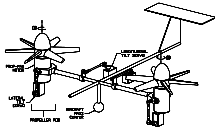
\includegraphics[width=0.7\textwidth]{figs/dualaxistilt}
\caption{General structure for opposed tilting platform, taken from\cite{gres2007}}
\label{fig:dualaxistilt}
\end{figure}
Research into birotor vehicles (Fig:\ref{fig:dualaxistilt}) with ancilliary lift propeller actuation is often termed \emph{Opposed Active Tilting} or \emph{OAT}. Such a rotorcraft's mechanical design applies either a single \emph{oblique} 45\textdegree ~tilting axis relative to the body \cite{smalltwotilting,obliquepitch}, or a \emph{lateral} tilting axis, adjacent to the body \cite{tiltrotorUAV,adaptivebackstep,tiltrotorcontrol,tpheonix}. Leading research is currently focussed on applying doubly actuated tilting axes to birotor UAVs. \emph{Dual} axis \emph{Opposed Active Tilting} or \emph{dOAT} introduces vectored thrust with independent propeller pitch and roll actions to further expand the actuation suite \cite{gres2007,opposedlateraldualaxis}. A birotor is sometimes considered preferable to higher degree of freedom multirotor platforms due to its reduced controller effort, however the controller plant derivation (typically requiring feedback linearization and virtual plant abstraction) often detracts from the quality and effectiveness of its stability solution as a result of the birotor's underactuation. 
\par
Birotor attitude control mostly introduces plant independent PD \cite{obliquepitch} and PID \cite{tiltrotorUAV} stabilizing controller schemes. Sometimes more computationally intensive and plant dependent \emph{ideal} or \emph{adaptive} backstepping controllers are implemented, presented in \cite{smalltwotilting,tpheonix} and \cite{adaptivebackstep} respectively. The gyroscopic response of a birotor vehicle's attitude system is more pronounced than that of a quadrotor, derived in Sec:\ref{sec:dynamics.nonlinearities}, and so feedback linearisation is almost always used. In an interesting progression from the norm, \cite{autopilotPSO} proposed an unique PID co-efficient selection algorithm for a bi-rotor control block. Using a particle swarm optimization (\emph{PSO}) technique, similar to \cite{adaptivepso}, the coefficients were globally optimized around a given performance metric. Their performance criterion is a standard integral time-weighted absolute error (\emph{ITAE}) term and nothing more appropriate involving effects unique to flight systems was used. \emph{PSO} algorithms iteratively search for a globally optimized solution and offer independent, gradient free based optimization. In subsequent chapters, controller coefficients are optimized for this project using PSO algorithms, shown later in Sec:\ref{sec:simulation.tuning}.
\par
\subsubsection*{Quadrotors}
Expanding on bi-rotor vehicles, the quadrotor UAV is a popular and well researched multirotor platform due to its mechanical simplicity. The current popularity of quadrotors as research platforms started in 2002 with a control algrithm implemented on what is now known as the X4-Flyer quadrotor \cite{x4flyer,x4flyercontrol}. Alternative iterations then followed; like the Microraptor\cite{microraptor} and STARMAC\cite{starmac} quadcopters which have subsequently been built and tested. A plethora of literature exists around quadrotor kinematics and their control \cite{dynamicmodelling2013, quaddynamics, fullquadcoptercontrol}, however dedicated rigid body 6-DOF mechanical derivations \cite{rigidbodylecture,eulerrigidbody} offer better explanations of the kinematics. Often the plant's dynamics are simplified around an origin trim point and assumed to reduce to six SISO plants for each degree of freedom (App:\ref{app:equations.standard}). Recent research projects have begun to incorporate nonlinear aerodynamic effects like drag and propeller blade-element momentum (\emph{BEM}) theory into the plant model\cite{lowreynolds,bem,starmac,nonlineardynamics}. The higher fidelity models for thrust and propeller responses offer more precision as they make fewer linearisations and assumptions.
\par
\begin{figure}[hbtp]
\centering
\begin{subfigure}{.5\textwidth}
\centering
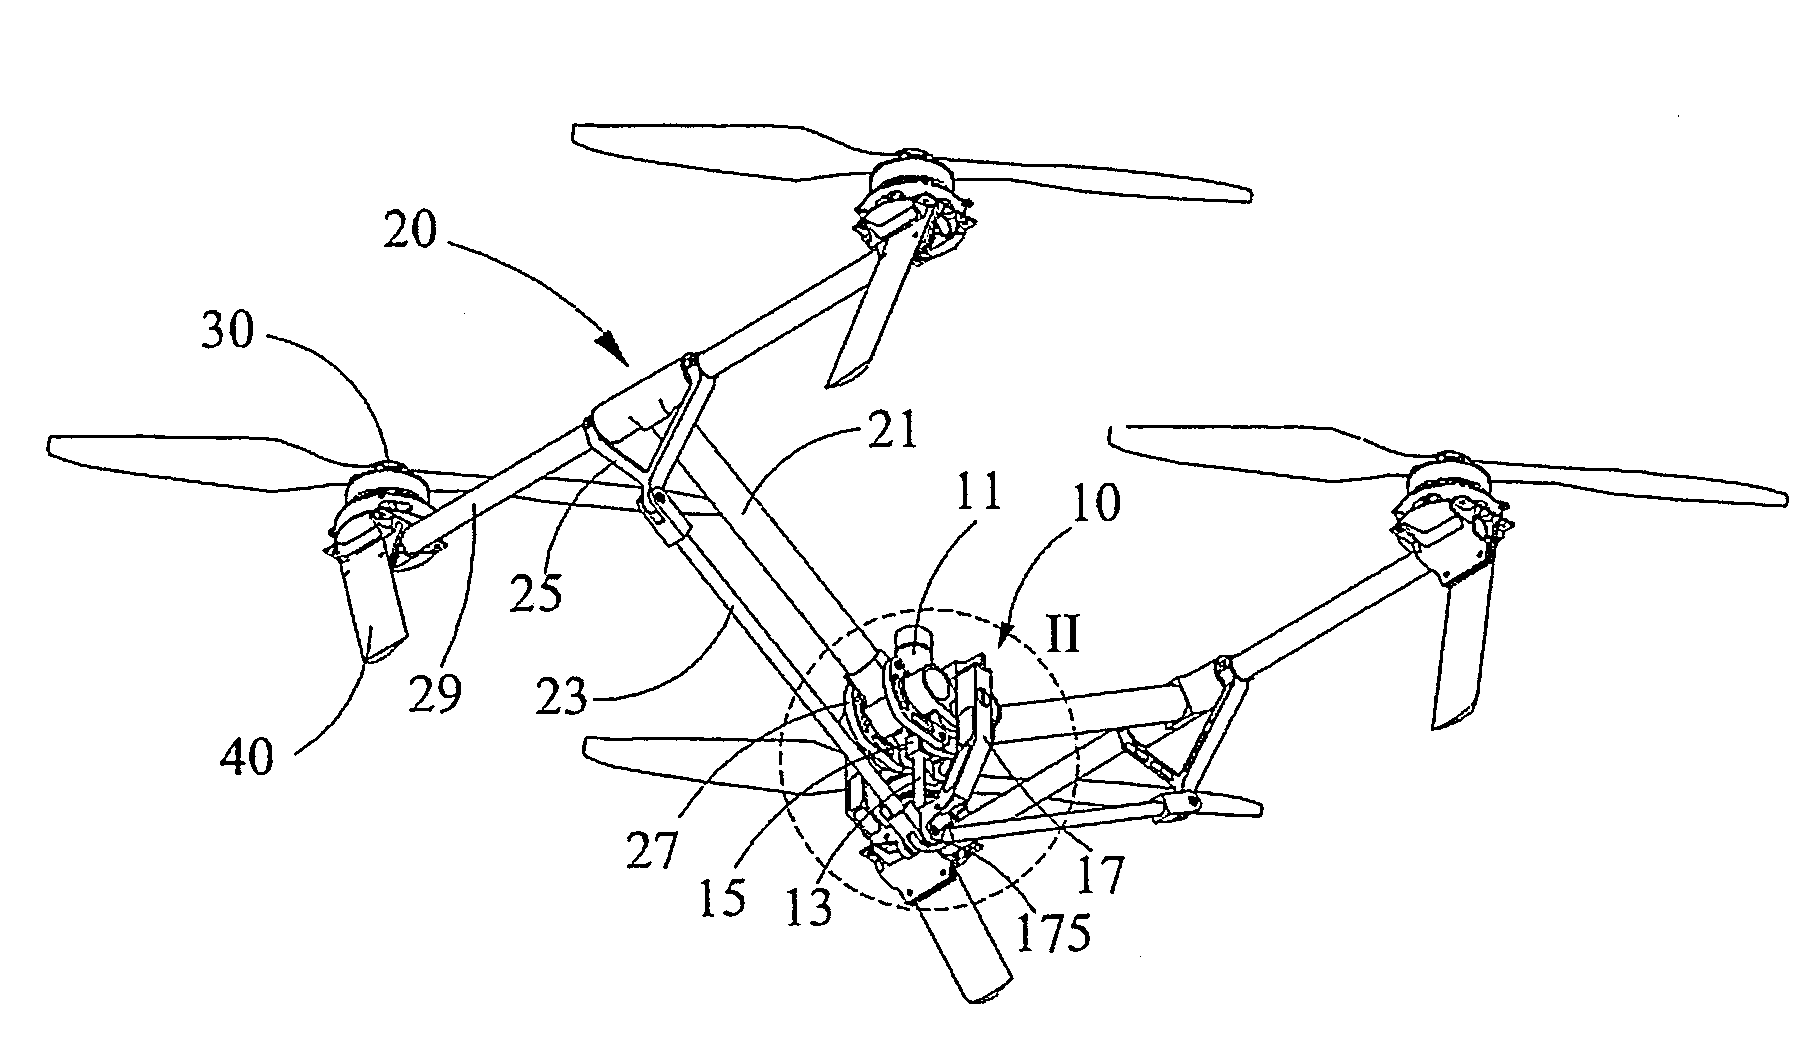
\includegraphics[width=\textwidth]{figs/dji-inspire1}
\caption{Inspire1 articulated upwards}
\label{fig:inspireup}
\end{subfigure}%
\begin{subfigure}{.5\textwidth}
\centering
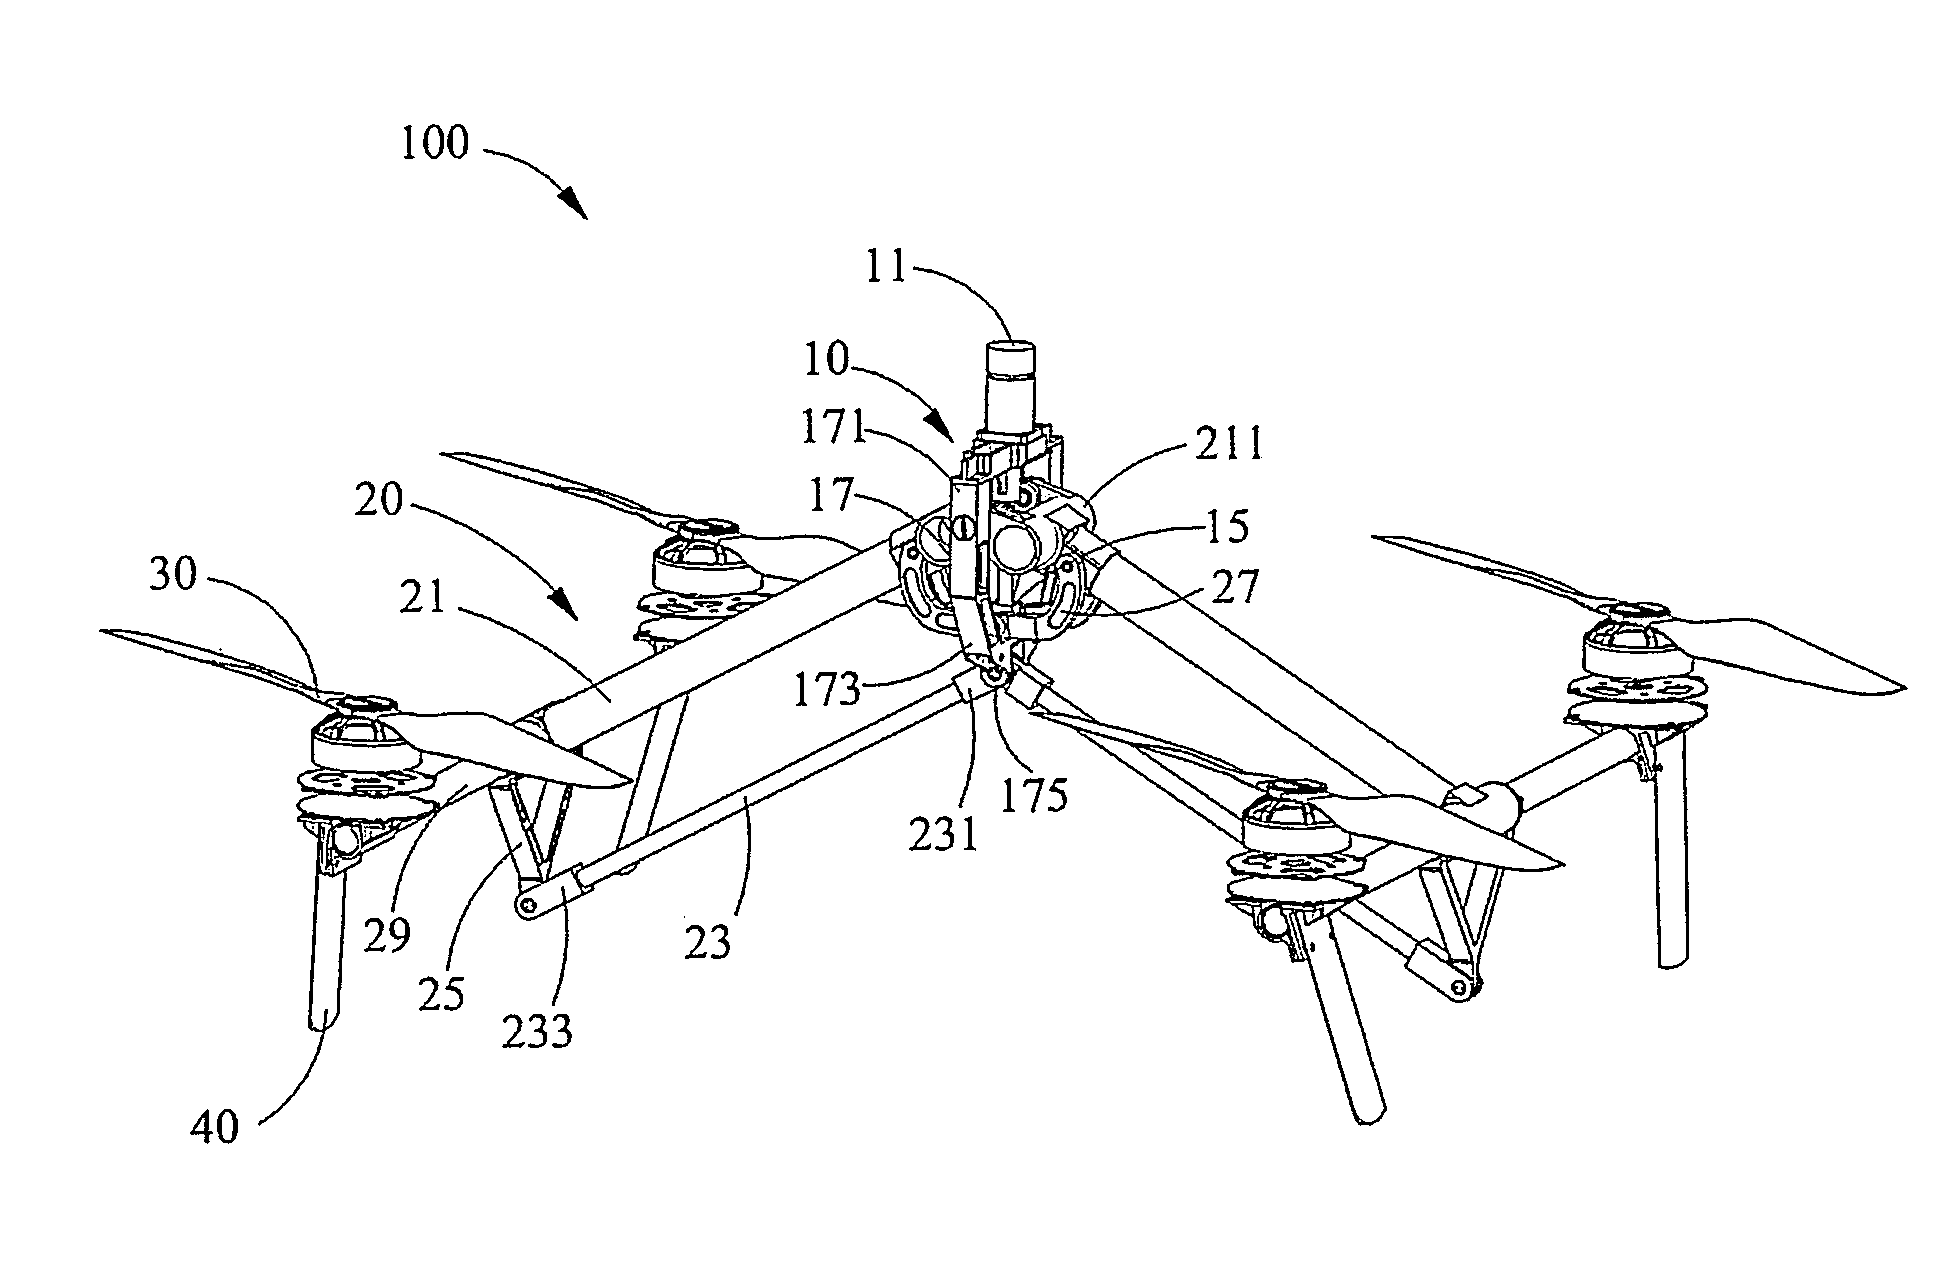
\includegraphics[width=\textwidth]{figs/dji-inspire2}
\caption{Inspire1 articulated downwards}
\label{fig:inspiredown}
\end{subfigure}
\caption{DJI Inspire1, the notations are with regards to the DJI patent \cite{djinspire}}
\label{fig:inspire1}
\end{figure}
At the time of writing, the only commercial UAV multirotor capable of structural transformation is the DJI Inspire1 quadrotor\cite{inspire}, manufactured by Shenzen DJI Technologies. DJI are better known for their hugely successful DJI Phantom commercial quadrotor\cite{phantom}. The Inspire1 can articulate its supporting arms up and down as shown in Fig:\ref{fig:inspire1}, the purpose of which is to both alter the center of gravity and to further expose a belly mounted camera gimbal for panoramic viewing angles. This changes the body's inertial matrix about its center of gravity, affecting the second order inertial response opposed to changes in angular velocity $\vec{\tau}=J\dot{\vec{\omega}}$. Variable inertia is a detrimental consequence which makes researchers apprehensive of reconfigurable aerospace frames. The range of transformations which the Inspire1 frame can undergo is limited to just articulating its arms up and down.
\par
In a similar fashion to the progression seen in birotor state-of-the-art, quadrotor research is engaging the topics of single and dual axis propeller tilting articulations. The extra actuation scheme(s) were first conceptualized and implemented on a prototype related to an ongoing project covered in two reports \cite{tiltpropellercontrol,tiltpropellerflight}. Those authors modified and tested a QuadroXL four rotor helicopter, produced by MikroKopter \cite{mikrokopter}, to actuate a single axis of tilting aligned with the frame's arms (Fig:\ref{fig:tiltpropellercontrol1}). Their proposed control solution, detailed next in Sec:\ref{subsec:intro.lit.control}, assumes no nominal linearised conditions around hover flight, unlike a similar single axis tilting quadrotor prototype presented in \cite{singleaxistilting}. The latter is \emph{simulated} but remains as yet untested.
\par
One approach to improving quadrotor flight response is to alter the manner in which the thrust is mechanically actuated, potentially improving actuator bandwidth (demonstrated in \cite{tiltgasco,tiltrihani}). Drawing from helicopter design, \cite{napsholm} purported a novel quadrotor UAV prototype that used swashplates for varying the propeller pitch and generating torque moments. The aim was a design which was independent of propeller rotational speed power electronics (\emph{ESCs}) for thrust force actuation.
\par
Petrol motors were intended for use in place of BLDC motors. Furthermore, the design proposed a single axis of tilt actuation to each of the four motor modules. Whilst mechanically complex, that prototype made use of existing off-the-shelf hobbyist helicopter components to design a rotor actuation bracket (Fig:\ref{fig:tiltrotor-napsholm}). The cyclic-pitch swashplates \cite{autonomousrobotspitch} used could apply pitching and rolling torques, $\tau_{\phi}$ and $\tau_{\theta}$, about each propeller's hub, its \emph{principle axis of rotation}. The torques were induced by cycling the blade's angle of attack throughout the propeller's rotational cycle. The actuation rate of such a configuration is far greater than that of a differential torque produced rolling/pitching motion.
\begin{figure}[htbp]
\begin{subfigure}{.5\textwidth}
\centering
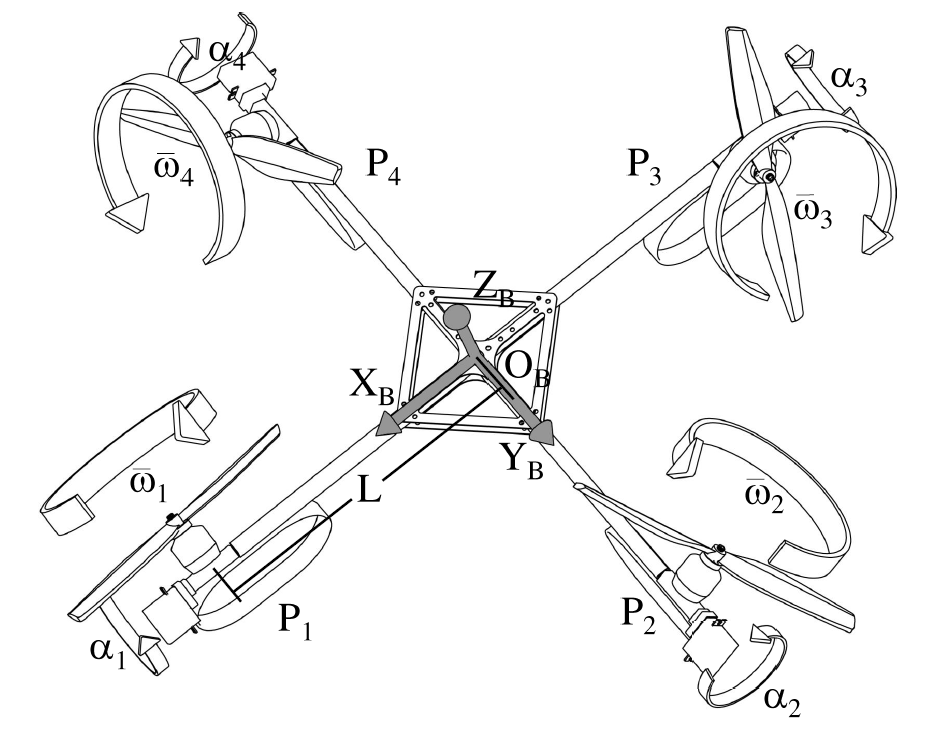
\includegraphics[width=0.9\textwidth]{figs/tiltpropellercontrol1}
\caption{Single aligned tilting axis, proposed in~\cite{tiltpropellercontrol}}
\label{fig:tiltpropellercontrol1}
\end{subfigure}%
\begin{subfigure}{.5\textwidth}
\centering
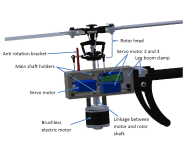
\includegraphics[width=0.9\textwidth]{figs/napsholm-mech}
\caption{Cyclic-pitch and swashplate mechanism from \cite{napsholm}}
\label{fig:tiltrotor-napsholm}
\end{subfigure}
\vspace{-4pt}
\caption{Tilt-rotor mechanisms}
\label{fig:tiltprop}
\vspace{-14pt}
\end{figure}
\par
Irrespective of the strong initial design in the early stages of \cite{napsholm}, it would appear that the research suffered due to time constraints. The introductory derivation on aerodynamic effects and deliberation over the design provide clear insight into the project's goals, however the control solution and system architecture are severely lacking in detail. A brief introductory proposal of an MPC attitude control system detracted from the comprehensive dynamics discussed. The project ended before testing, simulation or results could be obtained. Unfortunately, despite the novel overactuated design, there was no discussion about how the actuator allocation would be achieve.
\par
\begin{figure}[htbp]
\vspace{-12pt}
\centering
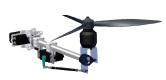
\includegraphics[width=0.68\textwidth]{figs/gasco-mech}
\vspace{-14pt}
\caption{Dual-axis tilt-rotor mechanism used in \cite{tiltgasco}}
\label{fig:tiltrotor-gasco}
\vspace{-10pt}
\end{figure}
Finally, the most crucial research to mention is \cite{tiltgasco}, which was a dual presented masters dissertation together with \cite{tiltrihani}. Currently, this appears to be the only project published pertaining to overactuation in aerospace bodies implemented and tested on a quadrotor platform. The research was split between the two authors who completed the electronic/control design and the mechanical design for their respective research projects. Shown in Fig:\ref{fig:tiltrotor-gasco}, the dual-axis articulation is achieved using an RC helicopter tail bracket and servo push-rod mechanism reducing the mass of the articulated components but limiting the range of its possible actuation. The propellers are treated as energy storing flywheels whose induced gyroscopic response act as a controllable actuator plant. Thrusts produced by the propellers were not vectored, but the controller's commanded virtual input is distributed to the actuator set by weighted pseudo-inversion, Sec:\ref{subsec:intro.lit.control}. The extra actuation is justified as fault tolerance redundancy (\emph{FTC}) but the project does not necessarily detail how such a redundancy could be beneficial.
%====================================================
\subsection{Notable Quadrotor Control Implementations}
\label{subsec:intro.lit.control}
%====================================================
\subsubsection*{Quadcopter Attitude Control}
%====================================================
\emph{\color{Gray}Note that here $\vec{\eta}$ is not necessarily an Euler angle set but any attitude representative state variable.}
\par
Attitude control of a 6-DOF aerospace body, quadrotor or otherwise, is best described by \cite{attitudecontrolproblem} and referred to as \emph{the attitude control problem}. For a rigid body that has an instantaneous (Euler) attitude state $\vec{\eta}_b$ and a desired state $\vec{\eta}_d$, the problem is to then find a stabilizing torque control $\vec{\tau}_\mu$. The control law is dependent on some feedback error state $\vec{\eta}_e$. Quaternion attitude states later replace Euler angles for attitude representation, $\vec{\eta}_b\Rightarrow Q_b$. A general attitude control law $h$ designs an input torque $\vec{\tau}_\mu$:
\begin{subequations}
\begin{equation} \label{eq:2}
\vec{\tau}_\mu \triangleq h(\vec{\eta}_d,\dot{\vec{\eta}}_d,\vec{\eta}_b,\dot{\vec{\eta}}_b,t)~~~~\in\mathcal{F}^b
\end{equation}
\vspace{-15pt}
\begin{equation}
=h(\vec{\eta}_e,\dot{\vec{\eta}}_e,t)~~\text{given some error state}~\vec{\eta}_e
\end{equation}
\end{subequations}
where the control law designs a net torque such that both the angular position and velocity rates are stabilized with the bounded limits; $\lim\vec{\eta}_b \rightarrow \vec{\eta}_d$ and $\lim\dot{\vec{\eta}}_b \rightarrow \dot{\vec{\eta}}_d$ respectively as $t \rightarrow \infty$. Stability definitions are expanded upon later in Sec:\ref{sec:control.stability}. A distinction must be made between euler angular rate vector $\dot{\vec{\eta}}_b=[\dot{\phi}~\dot{\theta}~\dot{\psi}]^T$ and the angular velocity vector $\vec{\omega}_b=[p~q~r]^T$. Depending on how the attitude is posed: with rotation matrices \cite{rigidbodylecture,eulerrigidbody,rotationsequences}, quaternions \cite{rotationsequences, spacecraftattitutdequaternions,fullquaternion} or otherwise (direct cosine matrix etc \ldots) the error state $\vec{\eta}_e= \vec{\eta}_d - \vec{\eta}_b$ could then differ to a (Hamilton) multiplicative relationship. \cite{attitudecontrolproblem} describes these conventionally different error states.
\par
Simulation and modelling papers often rely on Euler angle based rotation matrices for attitude representation, \cite{adaptivedisturbancecontrol, optimizedpidquadcopter, singleaxistilting, backsteppingquadcoptercontrol, fullquadcoptercontrol}, without addressing the inherent singularity associated with such an attitude representation (known as gimbal lock, \cite{euleranglesingularity}, Sec:\ref{subsec:dynamics.rigidbody.singularity}). The alternative quaternion attitude representation, first implemented in 2006 on a quadrotor UAV platform in \cite{attitudestabilization}, is often used in lieu of rotation matrices. Quaternions do have their own caveat of \emph{unwinding} as a result of the dual-coverage in $\mathbb{R}^3$ space, discussed in \cite{unwinding} and derived mathematically later in Sec:\ref{subsec:dynamics.rigidbody.unwinding}. Quaternions are $\in\mathbb{R}^4$ variables for attitude representations in $\mathbb{R}^3$ and so a mapping $\mathbb{R}^4\rightarrow\mathbb{R}^3$ produces an infinite coverage set for each unique attitude state in $\mathbb{R}^3$.
\par
Quadrotor plant dynamics are often simplified, especially when represented with a 3-variable Euler angle set, $\vec{\eta}_b = [\phi ~\theta ~\psi]^T$. The cross-coupled gyroscopic and Coriolis terms are both neglected when the body's angular velocity is small, $\vec{\omega}_b \approx \vec{0}$, and the inertial matrix $J_b$ is approximately diagonal, $rank(J_b)= x$ for $\in\mathbb{R}^x$. The consequence of such simplifications is the depreciation of both the gyroscopic torque term, $\vec{\tau}_{gyro}=-\vec{\omega}_b \times J_b\vec{\omega}_b \approx \vec{0}$ and the  Coriolis force term, $\vec{F}_{cor}=-\vec{\omega}_b \times m\vec{v}_b \approx \vec{0}$ in the body's dynamics~~(Ch:\ref{ch:dynamics} for context). 
\par
Once the coupled cross-product terms are no longer of consequence, the 6-DOF state trajectory, $\vec{\mathbf{x}}_b=[x ~y ~z ~\phi ~\theta ~\psi]^T$, can be treated as a series of independent SISO plants each controlled by an appropriate technique. Quaternion represented attitude plants cannot easily be decomposed into individual SISO channels (quaternion dynamics in Sec:\ref{subsec:dynamics.rigidbody.quaternion}). A quaternion combined four variable attitude state-space vector is then used, $Q_b \triangleq [q_0 ~\vec{q}\>]^T$, for the major loop trajectory plant of $\vec{\mathbf{x}}_b(t)$.
\begin{figure}[hbtp]
\vspace{-8pt}
\centering
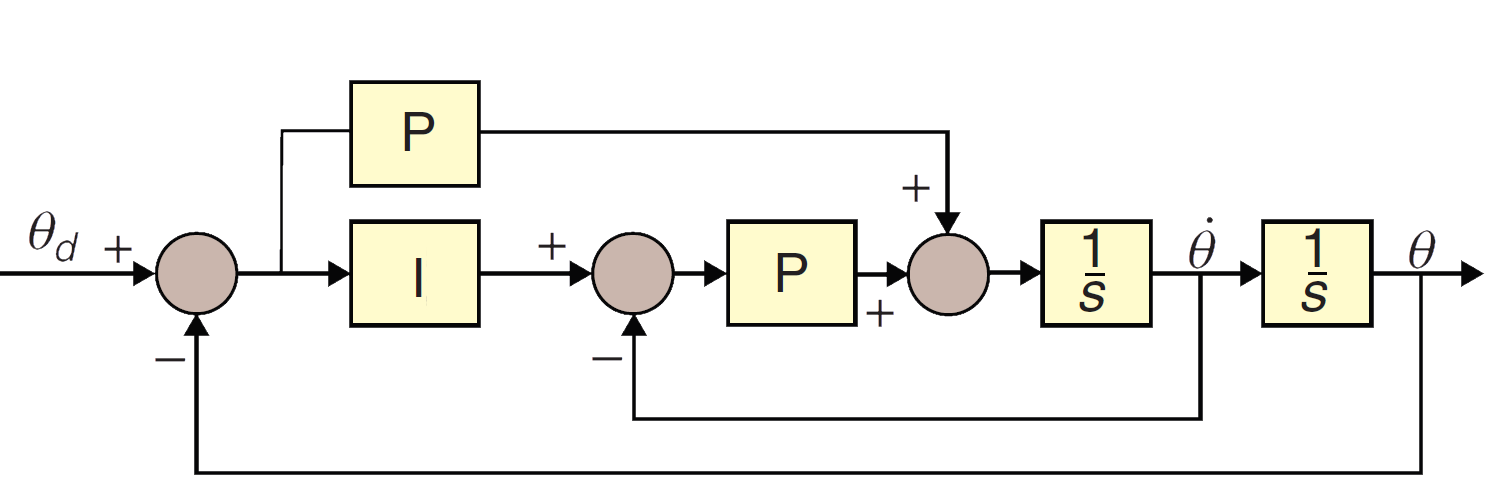
\includegraphics[width=0.75\textwidth]{figs/arducopter-pi}
\vspace{-2pt}
\caption{ArduCopter PI control structure for pitch angle channel $\theta$; from~\cite{buildyourownquad}}
\label{fig:arducopter-pi}
\vspace{-10pt}
\end{figure}
\par
Opensource and hobbyist flight controller software (Arducopter\cite{arducoptersite}, Openpilot\cite{openpilotsite} whose firmware stack is now maintained by LibrePilot, CleanFlight\cite{cleanflight}, BetaFlight\cite{betaflight}, etc \ldots) for custom fabricated UAV platforms all apply their own flavour of structured attitude controllers and state estimation algorithms, based on onboard hardware sensor fusion. \cite{buildyourownquad} summarizes the control structures implemented on a range of popular flight controllers. 
\par
The most popular of these, ArduCopter, implements a feed-forward PI compensation controller, whose single channel control loop for an attitude pitch channel $\theta$ is shown in Fig:\ref{fig:arducopter-pi}.  PI, PD and PID controllers are all popular and effective plant independent control solutions for general attitude plants. Table:\ref{tab:controllers} lists the common attitude control blocks (not exclusively quadrotors UAVs but MAVs too) and which projects they've been implemented in, after which a critique of the more unique adaptations is given. One ideal backstepping controller listed in Table:\ref{tab:controllers}, presented in \cite{tpheonix}, applies an algorithm derived through Hurwitz polynomials unlike the Lyapunov based backstepping control law(s) used here, derived later in Ch:\ref{ch:control}.
\begin{table}[h]
\centering
\begin{tabular}{ |c|l|l|c| }
\hline
Controller Type & Independent & Dependent & Total Examples\\ \hline
PI & \cite{attitudecontrolproblem} & \cite{attitudecontrolproblem} & 2\\ \hline
PD & \cite{tiltrihani} & \cite{fullquaternion,singleaxistilting} & 3\\ \hline
PID & \cite{optimizedpidquadcopter, attitudecontrolproblem, quaddynamics, tiltpropellercontrol, pidlqr} & \cite{attitudecontrolproblem, starmac, adaptivedisturbancecontrol} & 8\\ \hline
Lead & \cite{x4flyer} & N/A & 1\\ \hline
LQR & \cite{pidlqr} & N/A & 1\\ 
\hline
\multicolumn{3}{|c|}{Backstepping controllers} & \\
\hline
Ideal & \cite{tpheonix, backsteppingquadcoptercontrol} & \cite{backsteppingquadcoptercontrol} & 3\\ \hline
Adaptive & \multicolumn{2}{l|}{\cite{adaptivebackstep, nonlinearadaptive, 6dofbackstep, intelligentbackstep}} & 4\\ \hline
\end{tabular}
\caption{A breakdown of common attitude controllers}
\label{tab:controllers}
\end{table}
\par
\vspace{-15pt}
In a collection of papers, written by the most prolific early quadrotor authors S. Boubdallah and R. Siegward \cite{pidlqr,indoorslidingmode, fullquadcoptercontrol}, a range of different attitude control implementations is surveyed and tested on the OS4 platform. The final paper, \cite{fullquadcoptercontrol}, derived and pratically tested an integral backstepping attitude controller on the OS4 quadrotor platform. It builds on their research presented earlier in \cite{pidlqr} which provides an analysis of PID vs linear quadratic regulator (\emph{LQR}) attitude controllers, specifically in the context of underactuated quadrotor attitude control. LQR controllers aim to optimize the controller effort with actuator inputs $u\in\mathbb{U}$; controller effort is then $\norm{u}_2$ or the Euclidean norm (magnitude) of the plant input. Although, in theory, solving the associated Ricatti cost function may produce a cost optimal, stable and efficient control law, it needs exact plant matching. In reality, exact plant matching is difficult to achieve for a quadcopter or any aerospace body for that matter. The resultant controller in \cite{pidlqr} achieved asymptotic stability but had poor steady state performance due to low accuracy of the identified actuator dynamics and poor confidence inertial measurements.
\par
Adaptive Backstepping Control (in \cite{backstepping} or any other example in Table:\ref{tab:controllers}) expands on nominal ideal backstepping fundamentals by introducing disturbance and plant uncertainty terms into the Lyapunov energy function to be used for the backstepping suppression. For Lyapunov iteration, the adaptive backstepping process requires a disturbance estimate derivative or \emph{update law} which is often difficult to quantify. Approximation of plant disturbances without \emph{apriori} information is a complex subject. At some point in the design, an approximation heuristic must be adopted and that typically involves some compromise of performance over accuracy. One example of disturbance approximation in \cite{nonlinearadaptive} proposes using a statistical projection operator (or $proj(.)$, \cite{adaptiveregulation}). When used in adaptive control, presented similarly in \cite{outputfeedback}, the projection operator ensures a derivative based estimator can be bound for adaptive regression approximation{nonlinearregression}.
\par
Although the control implementation is not explicitly backstepping, in \cite{adaptiveslidingmode} a sliding mode controller was used to compensate for the disturbances in an Unmanned Submersible Vehicle attitude plant. The underwater current disturbances were approximated using a fuzzy logic system, specifically a \emph{zero-order Takagi-Sugeno-kang} fuzzy approximator. 
\par
The TSK system has been shown in \cite{zeroTSK} to mimic an artificial neural network approximator, where the fuzzy TSK system is more comprehensible than the latter. Statistical analysis and investigation of approximators without \emph{apriori} knowledge of a system are well beyond the scope of this research but are worth mentioning.
%====================================================
\subsubsection*{Single/Dual Axis Control \& Allocation}
\label{subsubsec:intro.lit.control.allocation}
%====================================================
The additional control actuation introduced with either single or dual axis articulation provides room for secondary control goals to be achieved. Of the few papers published on tilting-axis quadrotors, PD controllers (used in \cite{singleaxistilting} and again in both \cite{tiltgasco,tiltrihani}) and PID controllers (collectively \cite{tiltpropellercontrol,tiltpropellerflight}) are the standard fare for attitude control blocks. For either of these systems, there needs to be an allocation rule to distribute a commanded input amongst the actuator set. In a control allocation survery, \cite{allocation} describes the control allocation problem for a dynamic plant:
\begin{subequations} 
\vspace{-6pt}
\begin{equation} \label{eq:3.1}
\dot{\vec{\mathbf{x}}}=f(\vec{\mathbf{x}},t)+g(\vec{\mathbf{x}},\vec{\nu},t)~~~~~\vec{\mathbf{x}}\in\mathbb{R}^n,\vec{\nu}\in\mathbb{R}^m
\end{equation}
\vspace{-20pt}
\begin{equation} \label{eq:3.2}
\vec{y}=c(\vec{\mathbf{x}},t)
\end{equation}
\end{subequations}
\emph{\color{Gray} State variables of \cite{allocation} were changed to match this dissertation's conventions. In the state space equation Eq:\ref{eq:3.1}, it is assumed the plant input, $\vec{\nu}$, has a linear multiplicative relationship with the input response, $g(\vec{\mathbf{x}},t,\vec{\nu})\Rightarrow g'(\vec{\mathbf{x}},t)\vec{\nu}$. That linear relationship is a prerequisite for most allocation inversion rules but is not a necessity.}
\par
In Eq:\ref{eq:3.1} the state $\vec{\mathbf{x}}\in \mathbb{R}^n$ has associated plant dynamics $f(\vec{\mathbf{x}},t)$ and an input response $g(\vec{\mathbf{x}},\vec{\nu},t)$. Setpoint tracking control equates the output variable with the state, in practice only state estimates (denoted by a hat accent) are available:
\begin{equation}
\vec{y}=c(\vec{\mathbf{x}},t)=A(\vec{\mathbf{x}})=\hat{\mathbf{x}}
\end{equation}
Therefore the output $\vec{y}$ has the same dimension as the state variable $\vec{\mathbf{x}}$; or rather both $\vec{\mathbf{x}},\vec{y} \in \mathbb{R}^n$. In an ideal, well posed system the number of actuator inputs equals the number of outputs; that being $dim(\vec{\mathbf{x}})=dim(\vec{\nu})\in \mathbb{R}^n$ in the case where the control input $\vec{\nu}$ has a dimension $m$, for $m$ different actuator plants $\vec{\nu} \in \mathbb{R}^m$. If $m>n$ the problem is then overactuated and a level of abstraction is needed. The system mechanically commands a physical control input $\vec{\nu}_c$, dependent on explicit actuator positions $u\in\mathbb{U}\in\mathbb{R}^m$ as per some \emph{effectiveness} function derived from the actuator plant's dynamics:
\begin{equation}
\vec{\nu}_c=B(\vec{\mathbf{x}},u,t)~~~~\in\mathbb{R}^n
\end{equation}
where it is assumed that some higher level control law designs well a satisfactory stabilizing virtual control input from the error state(s) $\vec{\nu}_d=h(\vec{\mathbf{x}}_d,\dot{\vec{\mathbf{x}}}_d,\vec{\mathbf{x}}_b,\dot{\vec{\mathbf{x}}}_b,t)~\in\mathbb{R}^n$. The allocation rule then aims to solve for an explicit actuator position $u\in\mathbb{U}\in\mathbb{R}^m$ derived from $\vec{\nu}_d$ which actuates the physically commanded control input $\vec{\nu}_c$, minimizing the deviation or slack~$\vec{s}$ between virtual desired and physical commanded inputs $\vec{\nu}_d$ and $\vec{\nu}_c$ respectively. 
\par
Allocation is effectively a paradigm which transforms dimensions $\mathbb{R}^m\rightarrow\mathbb{R}^n$ using a commanded actuator matrix position $u\in\mathbb{R}^m$. An overactuated plant can be summarized into a nonlinear state space form as:
\begin{subequations}
\vspace{4pt}
\begin{equation} \label{eq:3.3}
\dot{\vec{\mathbf{x}}}=f(\vec{\mathbf{x}},t)+g(\vec{\mathbf{x}},\vec{\nu}_c,t)~~~~\vec{\mathbf{x}}\in \mathbb{R}^n
\end{equation}
\vspace{-12pt}
\begin{equation} \label{eq:3.4}
\vec{\nu}_c=B(\vec{\mathbf{x}},u,t)~~~~\vec{\nu}_c\in\mathbb{R}^n
\end{equation}
\vspace{-10pt}
\begin{equation}
\text{with}~u\in\mathbb{U}^m~\text{subject to some}~min(\vec{s}\hspace{3pt})~\text{such that}~\vec{s}=\vec{\nu}_d-\vec{\nu}_c
\end{equation}
\vspace{-10pt}
\begin{equation}
\text{using a generalized control law:}~\vec{\nu}_d=\mathcal{H}(\vec{\mathbf{x}}_d,\dot{\vec{\mathbf{x}}}_d,\vec{\mathbf{x}}_b,\dot{\vec{\mathbf{x}}}_b,t)~~~~\vec{\nu}_d\in\mathbb{R}^n
\end{equation}
\vspace{-10pt}
\begin{equation}
\vec{y}=c(\vec{\mathbf{x}},t)=\vec{\mathbf{x}}
\end{equation}
\end{subequations}
\par
The effectiveness function $B(\vec{\mathbf{x}},u,t)$ quantifies how actuator inputs $u\in\mathbb{U}$ correlate to the physically commanded plant input $\vec{\nu}_c$. Inversion based allocation rules which solve for explicit actuator solutions (Sec:\ref{sec:allocation.inversion}) require that $B(\vec{\mathbf{x}},u,t)$ can be abstracted to a linear multiplicative relationship $B'(\vec{\mathbf{x}},t)u$ with $B'(\vec{\mathbf{x}},t)\in\mathbb{R}^{n\times m}$, such that a generalized inverse of $B'(\vec{\mathbf{x}},t)$ can be found. For generic setpoint tracking the control law $\mathcal{H}$ will design a desired virtual control input $\vec{\nu}_d$, the allocation rule then has to solve $u$ for $\vec{\nu}_c$ such that for some slack variable $\vec{s}\triangleq\vec{\nu}_c-\vec{\nu}_d$ is minimized:
\begin{equation}\label{eq:quadraticallocator}
\underset{u \in \mathbb{R}^m,~s \in \mathbb{R}^n}{min}\norm{\vec{s}\hspace{2pt}}_2 ~\text{subject to} ~\vec{\nu}_c-\vec{\nu}_d=B(\vec{\mathbf{x}},u,t) - \mathcal{H}(\vec{\mathbf{x}}_e,\dot{\vec{\mathbf{x}}}_e,t)=\vec{s}~~~~u \in \mathbb{U}
\end{equation}
which ensures the commanded input $\vec{\nu}_c$ tracks the desired control input $\vec{\nu}_d$;~$\vec{\nu}_c\rightarrow\vec{\nu}_d$ as per some cost function of the slack variable . Mostly the L\textsubscript{2} norm $\norm{s}_2$ is used, but alternatively could be some different cost metric. In an overactuated system it then follows that there is a whole set of possible inputs for each commanded $\vec{\nu}_c$. An unique actuator solution (rather than a family of solutions) to Eq:\ref{eq:quadraticallocator} needs a secondary objective function, $j(\vec{\mathbf{x}},u,t)$ to be solved explicitly. Eq:\ref{eq:quadraticallocator} expands to:
\begin{equation} \label{eq:quadraticallocatorcost}
\underset{u \in \mathbb{R}^m,~s \in \mathbb{R}^n}{min}(\norm{\vec{s}}_2+j(\vec{\mathbf{x}},u,t)) ~\text{subject to} ~\vec{\nu}_c - \vec{\nu}_d=s~~~~u \in \mathbb{U}
\end{equation}
\par
The same author from \cite{allocation,efficientallocation,adaptiveallocation} proposed multiple control allocation solutions to a variety of systems. Following \cite{allocation}, in a subsequent paper \cite{efficientallocation}, the authors introduced a secondary cost function, driving the solution away from the typical linear quadratic programming pseudo and weighted inverse solutions.  Aiming for actuator efficiency and not just input saturation, a subsequent paper \cite{adaptiveallocation} proposed adaptively allocating actuator positions online. Using a Lyapunov energy equation as the online cost function, the minimization adaptive law settles to a feasible solution.
\par
Overactuation is not often applied to quadrotors and rather than providing a comprehensive literature review of associated papers here (which are all mostly theoretical derivation), the contextual application and solutions are expanded upon later in Ch:\ref{ch:allocation}. The only overactuated quadrotor literature which covers allocation of the extra actuators is \cite{tiltgasco,tiltrihani}, where the authors apply a weighted pseudo inverse (otherwise known as the Moore-Penrose Inverse \cite{moorepenrose}) allocation rule. Birotor dual-axis tilting, detailed earlier, results in a critically actuated system and so requires no allocation. As mentioned before, a prerequisite for (\emph{pseudo}) inversion is a multiplicative \emph{linear} control effectiveness relationship for Eq:\ref{eq:3.4}. 
\par
The only overactuated quadcopter paper which addressed its required control allocation was that of the combined project in \cite{tiltgasco,tiltrihani}. That proposed solution applied weighted inversion, relying on some very specific assumptions to achieve the required input actuator linearity for the system in Eq:\ref{eq:3.4}. The gyroscopic torque response to extra actuator $\eta$ pitching or $\gamma$ rolling movement, applied to each rotating propeller about the body's $\hat{X}_b$ and $\hat{Y}_b$ axes respectively, gives:
\begin{equation}\label{eq:1.10}
\vec{\tau}=\big(\dot{\eta}\cdot\hat{X}_b\big)\times J\big(\Omega\cdot\hat{Z}_b\big)~~\in\mathcal{F}^b
\end{equation}
with $\Omega$ being that propeller's rotational speed and $\dot{\eta}$ being the inducing servos rate. Projections onto body axes were used in Eq:\ref{eq:1.10} because the resultant thrust/responses were not vectored or assumed to be redirected. The authors assumed the extra actuators pitch and roll angular rates; $\dot{\eta}$~and~$\dot{\gamma}$ respectively, were both proportionally related to their positions $\eta$ and $\gamma$ as follows:
\begin{equation}
\dot{\eta}\approx \frac{1}{t_{settle}}\Delta\eta~~\text{and}~~\dot{\gamma}\approx \frac{1}{t_{settle}}\Delta\gamma
\end{equation}
where $t_{settle}$ is a constant derived in the actuator transfer function's settling time from a unit input step. Such an assumption holds true so long as $\Delta\eta$ or $\Delta\gamma$ is smaller than the initial step used to evaluate $t_{settle}$, a restrictive and unrealistic assumption but implemented nonetheless. It then follows that the gyroscopic first order torque $\vec{\tau}=-\vec{\omega}_b\times J_b\vec{\omega}_b$ and second order inertial torque $\vec{\tau}=J_b\dot{\vec{\omega}}_b$ responses are both functions of their associated servo positions $\eta$ and $\gamma$ and not theor respective derivatives. The extent of that consequence is contrasted with the allocation solution proposed later in Ch:\ref{ch:allocation}.
%====================================================
\subsubsection*{Satellite Attitude Control}
%====================================================
Unconstrained attitude setpoint tracking for 6-DOF bodies, quaternion based or otherwise, is a topic well covered in the field of satellite attitude control \cite{axissymmetricspacecraft, satellitebackstepping,lpvbackstepping}. The \emph{status quo} for recent research is on nonlinear adaptive backstepping attitude control systems, wherein the adaptive update rule is the novel contribution. Plant uncertainty always adversly affects the confidence in inertial measurements critical to the attitude control of a satellite. In \cite{lpvbackstepping} the authors proposed applying adaptive backstepping to compensate for steady state plant uncertainty errors of the (asymmetric) inertial estimations. 
\par
Alternatively, instead of deliberating on costly non-orbital prelaunch inertial measurements, \cite{inertiaestimation} suggested an algorithm for estimating the inertial matrix using controlled single axis perturbations. Such an approach does assume any initial values are sufficiently close to true body measurements such that estimates will settle and stability can be ensured, irrespective of how unacceptable the transient performance may be.
\par
Satellite actuator suites mostly include additional redundant effectors, to ensure fault tolerance, and thus require control allocation. Often the extra allocators are control moment gyroscopic actuators (flywheels driven by DC motors) to produce rotational torques. Thrusters have a limited amount of fuel and can actuate the system only a finite number of times. The thrusters can then be scheduled with a lower priority, preferring bias of electronic CMG actuators. In \cite{satellitebackstepping} the authors address the overactuation with direct pseudo inversion before applying quaternion based backstepping for attitude control. Such an inversion solves for Eq:\ref{eq:quadraticallocatorcost} as follows:
\begin{subequations}\label{eq:pseudoinv}
\vspace{4pt}
\begin{equation}\label{eq:pseudoinva}
u=B^{\dagger}\vec{\nu}_d
\end{equation}
\vspace{-12pt}
\begin{equation}\label{eq:pseudoinvb}
B^\dagger=B^T(BB^T)^{-1}
\end{equation}
\vspace{-10pt}
\begin{equation}
u\in\mathbb{R}^m,~\vec{\nu}_d\in\mathbb{R}^n,~B\in\mathbb{R}^{m\times n},~B^\dagger\in\mathbb{R}^{n\times m}
\end{equation}
\end{subequations}
where $B$ is the effectiveness matrix which is a static effector form of the effectiveness function $B(\vec{\mathbf{x}},u,t)$. The generalized inverse $B^{\dagger}$ is such that $BB^{\dagger}\equiv\mathbb{I}_{n\times n}$. Specifically $B^{\dagger}$ is the general \emph{pseudo} inversion matrix of $B$ (inversions included in Ch:\ref{ch:allocation}). Moreover there is an assumed \emph{affine} multiplicative relationship between the input, $u\in\mathbb{U}$, and the input effectiveness matrix from Eq:\ref{eq:3.4}. 
\par
The higher level controller designs actuator torques, $\vec{\nu}_d$, which are then used to solve for explicit actuator positions $u$ as per the inversion equation Eq:\ref{eq:pseudoinva}. Much like the overactuation previously discussed with respect to quadcopters; the pseudo inversion method of actuator distribution applies linear quadratic programming optimization to the allocation slack cost function, Eq:\ref{eq:quadraticallocator}. The resultant quaternion attitude backstepping controller developed in \cite{satellitebackstepping} demonstrated global uniform asymptotic stability. The strength of that backstepping stability lies in the choice of trajectory aiming to be stabilized; $z\rightarrow\vec{0}$. 
\par
The first candidate Lyapunov trajectory was defined as:
\begin{subequations}
\begin{equation}\label{eq:quaternion-trajectory.a}
z_1=\begin{bmatrix}
1-|q_0|\\
\vec{q}_e
\end{bmatrix}
\end{equation}
such that the Lyapunov energy function candidate is always positive definite and its derivative is positive definite descrescent. The particulars of that stability proof are omitted but it is worth detailing their chosen candidate function:
\begin{equation}
V_1(z)=z_1\text{}^Tz_1>0~~~~\forall[q_0,\vec{q}_e]
\end{equation}
\end{subequations}
The absolute quaternion error scalar used in Eq:\ref{eq:quaternion-trajectory.a} ensures a global trajectory's asymptotic stability (Sec:\ref{subsubsec:control.attitude.nonlinear.idealbackstep}), not just local stability that would otherwise be gained. The stable equilibrium points at $Q_e=\begin{bmatrix}
\pm 1 & \vec{0}~
\end{bmatrix}^T$ apply settling of the trajectory's \emph{error}, allowing the satellite to track its setpoint. Considering that the controller is an ideally compensating controller, the disturbance rejection and uncertainty compensation of the attitude controller could potentially disrupt that achieved stability. This was not discussed in the original paper.